\documentclass[landscape]{article}
\usepackage[pdftex]{graphicx}
\usepackage{rotating}
\pagestyle{empty}
\oddsidemargin  -0.5 in
\evensidemargin -0.5 in
\headheight     0 in
\topmargin      -1 in
\textheight     7.7 in
\textwidth      10 in
\newenvironment{slide}{\mbox{ }\vfill}{\vfill \mbox{ } \pagebreak}
\newenvironment{lastslide}{\mbox{ }\vfill}{\vfill \mbox{ }}
\begin{document}
\huge
\renewcommand{\labelitemi}{-}
\setlength{\parindent}{0 cm}

\begin{slide}
  \vfill
  \begin{center}
    \Huge Precise Measurement of $\Upsilon(1S,2S,3S)$ $\Gamma_{ee}$ in CLEO-III
  \end{center}

  \vfill
  \begin{center}
    Jim Pivarski
  \end{center}
  \vfill
\end{slide}

\begin{slide}
What is $\Upsilon(1S,2S,3S)$ $\Gamma_{ee}$?

\vfill
$e^+e^-$ contribution to $\Upsilon$ decay width: $\Gamma_{ee}$ = $\mathcal{B}_{ee} \times \Gamma$

\vfill
Related to the shape of the $b\bar{b}$ wavefunction: $\Gamma_{ee}$ = $\displaystyle \left(\frac{16 \pi {\alpha_{QED}}^2}{3 {M_\Upsilon}^2}\right) | \psi(0) |^2$

\vfill
\begin{center}
  \begin{tabular}{p{2 cm} p{9.9 cm} p{3.5 cm}}
    \begin{minipage}{\linewidth}
      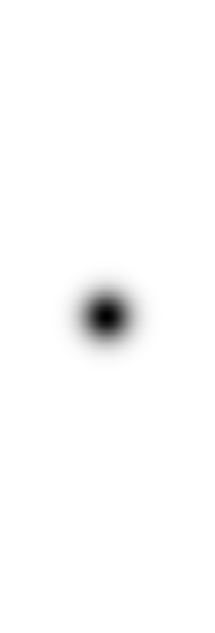
\includegraphics[height=5 cm]{fuzzytight}
    \end{minipage} & 
    \begin{minipage}{\linewidth}
      decays to $e^+e^-$ more readily than
    \end{minipage} & 
    \begin{minipage}{\linewidth}
      \includegraphics[height=5 cm]{fuzzyloose}
    \end{minipage}
  \end{tabular}
\end{center}

\vfill Therefore, it characterizes the strength of $b\bar{b}$ binding:

\vspace{0.5 cm}
\mbox{\hspace{12 cm}} how big an $\Upsilon$ the QCD potential permits

\end{slide}

\begin{slide}
Why measure $\Gamma_{ee}$ to high precision ($\sim$ 2\%)?

\vfill
It can be calculated on the lattice without ``quenching'': \\
this is a test of precision lattice gauge theory

\vfill
Also notice the similarity between
\begin{center}
  \begin{tabular}{l p{0.5 cm} p{9 cm} p{0.5 cm} r}
    \Huge $\Gamma_{ee}$: & &
    \begin{minipage}{\linewidth}
      \includegraphics[width=\linewidth]{gamee_diagram3}
    \end{minipage} & & \Huge and \\
    & & & & \\
    \Huge $f_B$: & &
    \begin{minipage}{\linewidth}
      \includegraphics[width=\linewidth]{fb_diagram3}
    \end{minipage} & &
  \end{tabular}
\end{center}

\vfill Experimental verification of $\Gamma_{ee}$ lends credence to
calculation of $f_B$.

\end{slide}

\begin{slide}
Best-kept secret about $\Gamma_{ee}$ measurement: uses $e^+e^- \to
\Upsilon$, not $\Upsilon \to e^+e^-$!

\vfill
\[ \Gamma_{ee} = \left(\frac{{M_\Upsilon}^2}{6 \pi^2}\right) \int \sigma(e^+e^- \to \Upsilon) \, dE \]

\vfill
\begin{center}
  \begin{tabular}{l p{0.95\linewidth}}
    \begin{rotate}{90}\mbox{\hspace{0.8 cm}} \LARGE Cross-section (arbitrary units)\end{rotate} &
      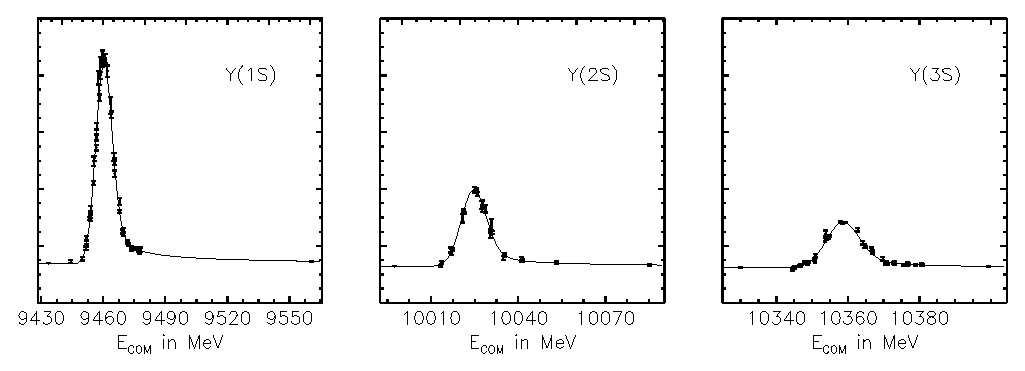
\includegraphics[width=\linewidth]{onetwothree}
  \end{tabular}
\end{center}

\vfill
So it's mostly a hadron count: the $e^+e^-$ final state is treated as a background
\end{slide}

\begin{slide}
Things that need to be very precise:

\vspace{-1.5 cm}
\renewcommand{\arraystretch}{2}
\begin{center}
  \begin{tabular}{c c p{0.5\linewidth} c c c}
    & & & $\Upsilon(1S)$ & $\Upsilon(2S)$ & $\Upsilon(3S)$ \\
    & 1. & \begin{minipage}{\linewidth} Statistical uncertainty \\ (dominated by $e^+e^- \to \gamma\gamma$ counting) \end{minipage} & 0.4 -- 0.7\% & 1.0 -- 1.6\% & 1.0 -- 2.4\% \\
    $\surd$ & 2. & Background subtraction & $\longleftarrow$ & 0.3\% & $\longrightarrow$ \\
    $\surd$ & 3. & Search for bad runs & & & \\
    $\surd$ & 4. & \begin{minipage}{\linewidth} Radiative corrections and continuum \\ interference (Karl Berkelman) \end{minipage} & 0.2\% & 0.2\% & 0.2\% \\
    & 5. & Beam energy-calibration jitter? & $\longleftarrow$ & 1\% ? & $\longrightarrow$ \\
    $\surd$ & 6. & Hadronic efficiency & 1.1\% & 1.4\% & 1.3\% \\
    $\surd$ & 7. & $(1-3\mathcal{B}_{\mu\mu})$ for total $\sigma$ (Istvan Danko) & $\longleftarrow$ & 0.1\% & $\longrightarrow$ \\
    & 8. & \begin{minipage}{\linewidth} Luminosity (Surik Mehrabyan,
    \\ Brian Heltsley, and sometimes me) \end{minipage} & $\longleftarrow$ & 2\% ? & $\longrightarrow$ \\
  \end{tabular}
\end{center}
\end{slide}

\begin{slide}
{\bf Backgrounds:} all continuum processes are subtracted in the fit, \\
non-beam-beam backgrounds are subtracted run-by-run

\vfill
\begin{center}
  \includegraphics[width=0.9\linewidth]{backgrounds}
\end{center}

\end{slide}

\begin{slide}
{\bf Search for bad runs:} lots of methods, most useful are trackless
bhabha fraction and events versus time

\vfill
\begin{center}
  \begin{tabular}{c p{0.9\linewidth}}
    \begin{rotate}{90}\mbox{\hspace{2 cm}} Number of trackless bhabhas\end{rotate} & \includegraphics[width=\linewidth, clip=true, bb=20 13 420 211]{../runbyrun_trackless2} \\
    & \vspace{-1 cm} \begin{center} Fraction of the event (0 = beginning, 1 = end) \end{center}
  \end{tabular}
\end{center}
\end{slide}

\begin{slide}
{\bf Search for bad runs:} found 64 beyond those in Dave Kreinick's
{\tt badruns3S}

\vspace{-1 cm}
\begin{center}
  \LARGE
  \renewcommand{\arraystretch}{3}
  \begin{tabular}{p{0.38\linewidth} p{0.6\linewidth}}
    \begin{minipage}{\linewidth} Cosmic ray backgrounds $>$ 5\% or \\ beam-gas backgrounds $>$ 2\% \end{minipage} &
    \begin{minipage}{\linewidth} 122353 126341 129522 \end{minipage} \\
    \begin{minipage}{\linewidth} Other large backgrounds \end{minipage} & \begin{minipage}{\linewidth} 121595 122093 122330 126510 \end{minipage} \\
    \begin{minipage}{\linewidth} BarrelBhabha trigger inefficiency \end{minipage} &
    \begin{minipage}{\linewidth} 121710 121928 121929 121930 121944 121953 121954 123884 127951
    127955 130278 \end{minipage} \\
    \begin{minipage}{\linewidth} Noisy (high-energy) showers in barrel \end{minipage} &
    \begin{minipage}{\linewidth} 122331 122335 122336 122339 122341 122342 122344 122345 122349
    122350 122352 \end{minipage} \\
    \begin{minipage}{\linewidth} DR lost sensitivity before end of run \\ (trackless bhabhas) \end{minipage} &
    \begin{minipage}{\linewidth} 121476 121748 121822 121847 122685 123436 123847 123873 124816
    124860 124862 125367 126273 126329 127280 \end{minipage} \\
    \begin{minipage}{\linewidth} Bhabha track momentum distribution \\ is abruptly wide \end{minipage} &
    \begin{minipage}{\linewidth} 124452 124454 124456 124458 124462 124464 124465 124466 124467
    124469 124472 124473 124474 124475 124477 124478 124479 124480 \end{minipage} \\
    \begin{minipage}{\linewidth} Hadronic cross-section plummets \\ in the last few minutes \end{minipage} &
    \begin{minipage}{\linewidth} 123281 123411 \end{minipage} \\
  \end{tabular}
\end{center}

\vfill
\end{slide}

\begin{slide}
{\bf Hadronic efficiency:}

\vfill
I define ``Hadronic decay'' to be ``anything but $\Upsilon \to e^+e^-$, $\mu^+\mu^-$, or $\tau^+\tau^-$.''

\vfill
Can't be certain that the Monte Carlo simulates all decays

\vfill
\renewcommand{\labelitemi}{\mbox{\large $\bullet$}} 
\begin{itemize}\setlength{\itemsep}{0.5 cm}

  \item Trigger efficiency is studied three different ways: MC's 99.6\% is given $\pm$1.0\% error

  \item MC cut efficiencies are tested in $\Upsilon(2S) \to \underbrace{\pi^+\pi^-} \Upsilon(1S)$ decays \\
    \mbox{\hspace{13 cm}} $\searrow$ \\
    \mbox{\hspace{12 cm}} \begin{minipage}{11.5 cm} \renewcommand{\arraystretch}{1}
      \begin{tabular}{l l}
	chosen to & satisfy trigger and L4 \\
	& satisfy event type filters \\
	& miss the calorimeter barrel \\
	& not ``curl'' in drift chamber
      \end{tabular}
      (acceptance independent of $\Upsilon(1S)$)
    \end{minipage}

  \item Each cut is assigned a systematic error from this data/MC comparison

  \item Assume MC is equally good at describing $\Upsilon(2S)$, $\Upsilon(3S)$ \\
    (verified by data in most of the parameter space)

  \item Propagate branching fraction uncertainties

\end{itemize}

\vfill
\end{slide}

\begin{slide}
{\bf Hadronic efficiency:} $\Upsilon(1S)$ from $\Upsilon(2S) \to \pi^+\pi^- \Upsilon(1S)$

\vfill
\begin{center}
  \includegraphics[width=0.7\linewidth, clip=true, bb=0 262 550 520]{../cascades_recoilmass}
  \includegraphics[width=0.7\linewidth, clip=true, bb=0 262 550 520]{../cascades_visen}
\end{center}
\end{slide}

\begin{slide}
{\bf Hadronic efficiency:} application of $\Upsilon(1S)$ MC validity to $\Upsilon(2S,3S)$

\vfill
\begin{center}
%  \includegraphics[width=0.9\linewidth, clip=true, bb=0 0 405 240]{../efficiency_overlay}
  \includegraphics[width=0.55\linewidth]{../efficiency_visen}
\end{center}
\end{slide}

\begin{slide}
{\bf Hadronic efficiency:} bottom line

\renewcommand{\arraystretch}{1.5}
\begin{center}
  \begin{tabular}{p{0.6\linewidth} c c c}
    & $\Upsilon(1S)$ & $\Upsilon(2S)$ & $\Upsilon(3S)$ \\\hline
    Trigger & 0.7\% & 1.0\% & 1.0\% \\
    Verification with $\Upsilon(2S) \to \pi^+\pi^- \Upsilon(1S)$ & 0.6\% & $\longrightarrow$ & $\longrightarrow$ \\
    Further verification with continuum-subtracted data & 0.3\% & 0.3\% & 0.3\% \\
    Branching fraction uncertainties & 0.01\% & 0.05\% & 0.04\% \\
    Monte Carlo errors & 0.5\% & 0.5\% & 0.4\% \\\hline
    Total uncertainty & 1.1\% & 1.3\% & 1.3\%
  \end{tabular}

  \vfill
  \begin{tabular}{p{0.6\linewidth} c c c}
    Total hadronic efficiency & 98.7\% & 96.7\% & 97.0\%
  \end{tabular}
\end{center}

\vfill
\end{slide}

%% 1-chi^2 probabilities for 1,2,3S continuum
%% {CDF[ChiSquareDistribution[124], 107.868433108],
%% CDF[ChiSquareDistribution[274], 259.141499129],
%% CDF[ChiSquareDistribution[125], 113.358624018]}
%% Out[2]= {0.151585, 0.268301, 0.236399}

%% reduced chi^2 for 1,2,3S continuum
%% Out[3]= {0.869907, 0.945772, 0.906869}

%% 1-chi^2 probabilities for 1,2,3S peak points
%% {CDF[ChiSquareDistribution[651], 705.080272442],
%%  CDF[ChiSquareDistribution[633], 740.061321596],
%%  CDF[ChiSquareDistribution[601], 546.798657484]}
%% Out[4]= {0.930231, 0.997966, 0.0555114}
  
%% reduced chi^2 for 1,2,3S peak points
%% Out[5]= {1.08307, 1.16913, 0.909815}

%% BUT for the 2S peak that you actually USE:
%% CDF[ChiSquareDistribution[262], 268.21]
%% P = 0.617241 and reduced chi^2 = 1.0237

\begin{slide}
{\bf Hadronic cross-section stability:}

\vfill
Reduced $\chi^2$ for fits to a constant cross-section

\vfill \renewcommand{\arraystretch}{1.25}
\begin{center}
  \begin{tabular}{p{0.4\linewidth} c c c}
    & $\Upsilon(1S)$ & $\Upsilon(2S)$ & $\Upsilon(3S)$ \\\hline
%%     off-resonance runs & 85\% & 73\% & 76\% \\
%%     on-resonance runs & 7\% & 38\% & 94\%
    off-resonance runs & 0.87 & 0.95 & 0.91 \\
    \#degrees of freedom & (124) & (274) & (125) \\\hline
    on-resonance runs & 1.08 & 1.02 & 0.91 \\
    \#degrees of freedom & (651) & (262) & (601)
  \end{tabular}
\end{center}

\vfill
Reduced $\chi^2$ for all-continuum fit to $1/s$ ($+$ tail corrections)
\mbox{\hspace{1.4 cm}}
\begin{tabular}{c}
%%    & & 20\% &
%%    & & 1.06 & \\
  \\
  0.98 \\
  (525)
\end{tabular}

\vfill
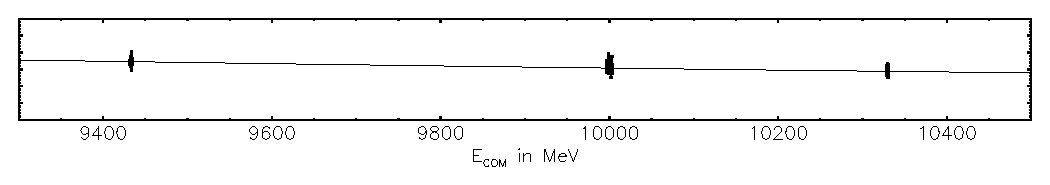
\includegraphics[width=\linewidth]{oneovers}
\end{slide}

\begin{slide}
{\bf Checklist:}

\vfill
\renewcommand{\arraystretch}{2}
\begin{center}
  \begin{tabular}{c c p{0.8\linewidth}}
    $\surd$ & 1. & Background subtraction \\
    $\surd$ & 2. & Search for bad runs \\
    $\surd$ & 3. & Hadronic efficiency (completely done) \\
    $\sim$ & 4. & Fit all scans (minor improvement in method needed) \\
    & 5. & Quantify beam energy-calibration uncertainty ($\sigma$ versus time) \\
    & 6. & Convert $e^+e^- \to \gamma\gamma$ count into luminosity \\
  \end{tabular}
\end{center}

\vfill
Barring disasters, you will see a 10-day CBX posting before next meeting

\end{slide}








\end{document}
